\section{Classificação de grafos}

\begin{frame}[fragile]{Simples, completo e subgrafos}

    \begin{itemize}
        \item Um grafo é dito simples se ele não contém \textit{autoloops} nem multiarestas

        \item Um grafo que não é simples é denominado multigrafo

        \item A maior parte dos grafos que modelam aplicações práticas são simples

        \item Um grafo é dito completo se, para cada par de vértices $u, v \in V, u \neq v$, 
            tem-se que $(u, v)\in E$

        \item O grafo $S(V', E') \subset G(V, E)$ é denominado subgrafo de $G$ se $V'\subset V,
            E'\subset E$ e, para qualquer par $(a, b)\in E'$, vale que $a, b \in V'$
    \end{itemize}

\end{frame}

\begin{frame}[fragile]{Visualização de um grafo simples completo, com um subgrafo $S$ em azul}

    \begin{figure}
        \centering

        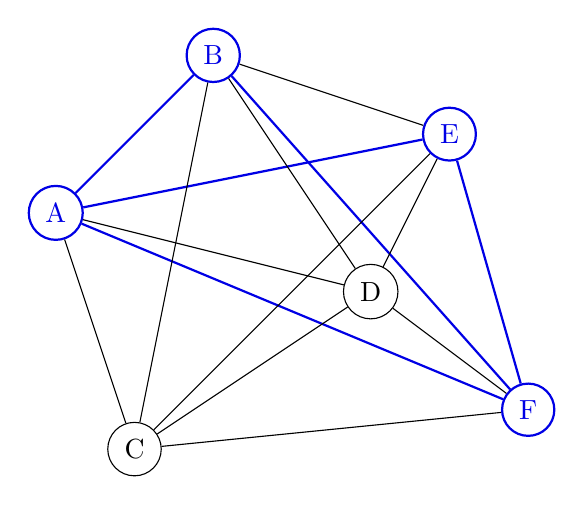
\begin{tikzpicture}
            \node[thick,blue!90!black,draw,circle] (A) at (0, 3) { A };
            \node[thick,blue!90!black,draw,circle] (B) at (2, 5) { B };
            \node[draw,circle] (C) at (1, 0) { C };
            \node[draw,circle] (D) at (4, 2) { D };
            \node[thick,blue!90!black,draw,circle] (E) at (5, 4) { E };
            \node[thick,blue!90!black,draw,circle] (F) at (6, 0.5) { F };

            \draw[thick,blue!90!black] (A) -- (B);
            \draw (A) -- (C);
            \draw (A) -- (D);
            \draw[thick,blue!90!black] (A) -- (E);
            \draw[thick,blue!90!black] (A) -- (F);
            \draw (B) -- (C);
            \draw (B) -- (D);
            \draw (B) -- (E);
            \draw[thick,blue!90!black] (B) -- (F);
            \draw (C) -- (D);
            \draw (C) -- (E);
            \draw (C) -- (F);
            \draw (D) -- (E);
            \draw (D) -- (F);
            \draw[thick,blue!90!black] (E) -- (F);
        \end{tikzpicture}

    \end{figure}

\end{frame}


\begin{frame}[fragile]{Grafos direcionados, ponderados e densos}

    \begin{itemize}
        \item Se, para qualquer aresta $(u, v)\in E$, vale que $(v, u)\in E$, o grafo é dito
            não direcionado

        \item Caso contrário, o grafo é direcionado, e a aresta $(u, v)$ significa que $u$ está
            relacionado a $v$, mas não necessariamento o contrário

        \item Se a cada aresta $e\in E$ for associado um valor $w$, denominado peso, o grafo é
            denominado grafo ponderado

        \item Um grafo que não tem pesos associados às arestas é chamado grafo não poderado

        \item Um grafo é dito esparso se o número de aresta $E$ é ``pequeno'' (em geral, $O(V)$)

        \item Um grafo é dito denso se o número de arestas $E$ é ``grande'' (em geral, $O(V^2)$)
    \end{itemize}

\end{frame}

\begin{frame}[fragile]{Visualização de um grafo esparso ponderado não direcionado}

    \begin{figure}
        \centering

        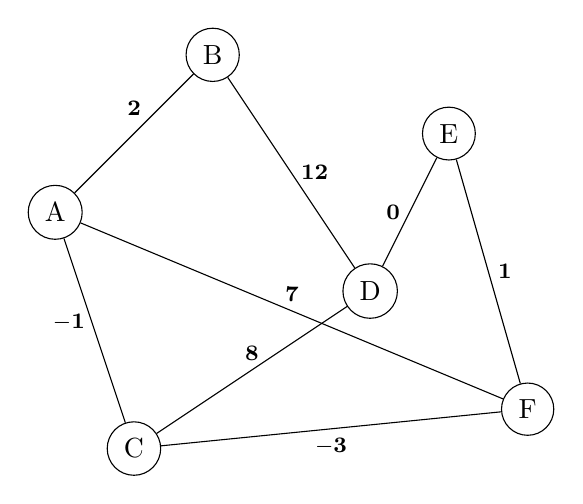
\begin{tikzpicture}
            \node[draw,circle] (A) at (0, 3) { A };
            \node[draw,circle] (B) at (2, 5) { B };
            \node[draw,circle] (C) at (1, 0) { C };
            \node[draw,circle] (D) at (4, 2) { D };
            \node[draw,circle] (E) at (5, 4) { E };
            \node[draw,circle] (F) at (6, 0.5) { F };

            \draw (A) -- node[anchor=south,yshift=0.1cm] { \footnotesize $\mathbf{2}$ } (B);
            \draw (A) -- node[anchor=east,yshift=0.1cm] { \footnotesize $\mathbf{-1}$ } (C);
            \draw (A) -- node[anchor=south,yshift=0.0cm] { \footnotesize $\mathbf{7}$ } (F);
            \draw (B) -- node[anchor=west,xshift=0.0cm] { \footnotesize $\mathbf{12}$ } (D);
            \draw (D) -- node[anchor=east,yshift=0.0cm] { \footnotesize $\mathbf{0}$ } (E);
            \draw (C) -- node[anchor=south,yshift=0.0cm] { \footnotesize $\mathbf{8}$ } (D);
            \draw (C) -- node[anchor=north,yshift=0.0cm] { \footnotesize $\mathbf{-3}$ } (F);
            \draw (E) -- node[anchor=west,yshift=0.0cm] { \footnotesize $\mathbf{1}$ } (F);
        \end{tikzpicture}

    \end{figure}

\end{frame}


\begin{frame}[fragile]{Visualização de um grafo denso, direcionado e não ponderado}

    \begin{figure}
        \centering

        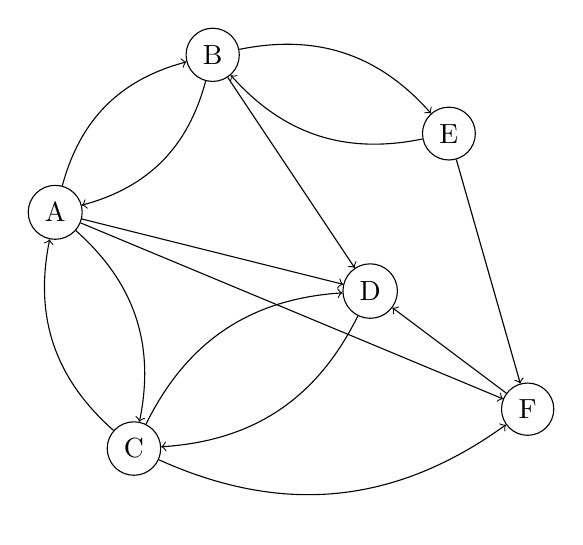
\begin{tikzpicture}
            \node[draw,circle] (A) at (0, 3) { A };
            \node[draw,circle] (B) at (2, 5) { B };
            \node[draw,circle] (C) at (1, 0) { C };
            \node[draw,circle] (D) at (4, 2) { D };
            \node[draw,circle] (E) at (5, 4) { E };
            \node[draw,circle] (F) at (6, 0.5) { F };

            \draw[->] (A) to [bend left] (B);
            \draw[->] (B) to [bend left] (A);
            \draw[->] (A) to [bend left] (C);
            \draw[->] (C) to [bend left] (A);
            \draw[->] (D) to [bend left] (C);
            \draw[->] (C) to [bend left] (D);
            \draw[->] (B) to [bend left] (E);
            \draw[->] (E) to [bend left] (B);




            \draw[->] (A) -- (D);
            \draw[->] (A) -- (F);
            \draw[->] (B) -- (D);
            \draw[->] (C) to [bend right] (F);
            \draw[<-] (D) -- (F);
            \draw[->] (E) -- (F);
        \end{tikzpicture}

    \end{figure}

\end{frame}


\begin{frame}[fragile]{Graus de chegada e de saída}

    \begin{itemize}
        \item O graup de entrada $g_i(u)$ de um vértice $u$ é igual ao número de arestas $e\in E$
            cuja segunda coordenada é igual a $u$

        \item Em outras palavras, é igual a o número de arestas que ``chegam'' em $u$

        \item De forma semelhante, o grau de saída $g_o(u)$ de um vértice $u$ é dado pelo número
            de arestas $e\in E$ tais que a primeira coordenada é igual a $u$

        \item Isto é, é o número de arestas que ``partem'' de $u$

        \item Em um grafo não-direcionado, $g_i(u) = g_o(u)$, $\forall u\in V$
    \end{itemize}

\end{frame}

\begin{frame}[fragile]{Visualização dos graus de chegada e saída}

    \begin{figure}
        \centering

        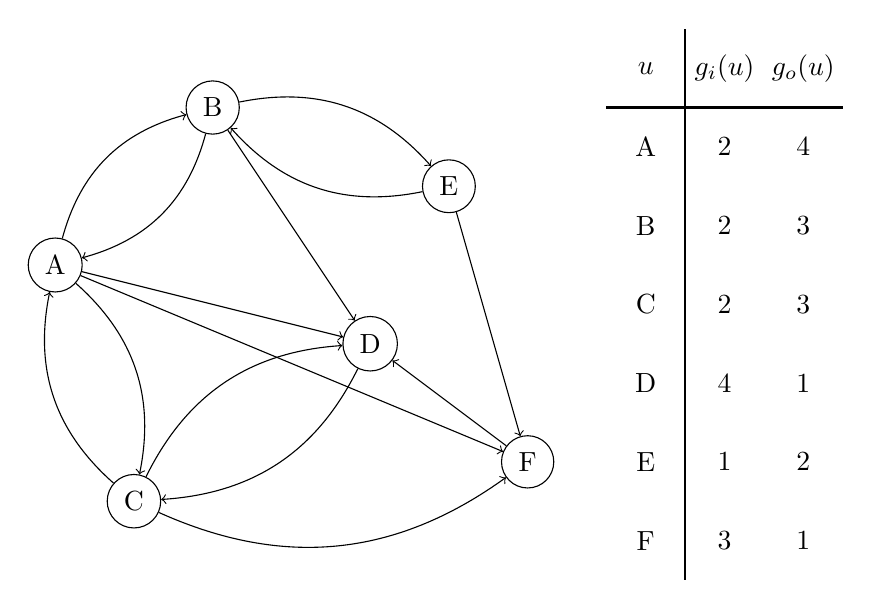
\begin{tikzpicture}
            \node[draw,circle] (A) at (0, 3) { A };
            \node[draw,circle] (B) at (2, 5) { B };
            \node[draw,circle] (C) at (1, 0) { C };
            \node[draw,circle] (D) at (4, 2) { D };
            \node[draw,circle] (E) at (5, 4) { E };
            \node[draw,circle] (F) at (6, 0.5) { F };

            \draw[thick] (8, -1) -- (8, 6);
            \draw[thick] (7, 5) -- (10, 5);

            \node at (7.5, 5.5) { $u$ };
            \node at (8.5, 5.5) { $g_i(u)$ };
            \node at (9.5, 5.5) { $g_o(u)$ };

            \node at (7.5, 4.5) { A };
            \node at (8.5, 4.5) { $2$ };
            \node at (9.5, 4.5) { $4$ };

            \node at (7.5, 3.5) { B };
            \node at (8.5, 3.5) { $2$ };
            \node at (9.5, 3.5) { $3$ };

            \node at (7.5, 2.5) { C };
            \node at (8.5, 2.5) { $2$ };
            \node at (9.5, 2.5) { $3$ };

            \node at (7.5, 1.5) { D };
            \node at (8.5, 1.5) { $4$ };
            \node at (9.5, 1.5) { $1$ };

            \node at (7.5, 0.5) { E };
            \node at (8.5, 0.5) { $1$ };
            \node at (9.5, 0.5) { $2$ };

            \node at (7.5, -0.5) { F };
            \node at (8.5, -0.5) { $3$ };
            \node at (9.5, -0.5) { $1$ };

            \draw[->] (A) to [bend left] (B);
            \draw[->] (B) to [bend left] (A);
            \draw[->] (A) to [bend left] (C);
            \draw[->] (C) to [bend left] (A);
            \draw[->] (D) to [bend left] (C);
            \draw[->] (C) to [bend left] (D);
            \draw[->] (B) to [bend left] (E);
            \draw[->] (E) to [bend left] (B);
            \draw[->] (A) -- (D);
            \draw[->] (A) -- (F);
            \draw[->] (B) -- (D);
            \draw[->] (C) to [bend right] (F);
            \draw[<-] (D) -- (F);
            \draw[->] (E) -- (F);
        \end{tikzpicture}

    \end{figure}

\end{frame}


\begin{frame}[fragile]{Caminhos}

    \begin{itemize}
        \item Um caminho entre dois vértices $u$ e $v$ é uma sequência de arestas que conectam
            ambos vértices

        \item Em outros termos, é uma sequência não-nula de arestas
        \[
            (u, w_1), (w_1, w_2), (w_2, w_3), \ldots, (w_{n-1}, w_n), (w_n, v),
        \]
        onde $u$ é o ponto de partida e $v$ o ponto de chegada

        \item Obserque, para quaisquer duas arestas consecutivas do caminho 
            $e = (e_1, e_2), f = (f_1, f_2)$, vale que $e_2 = f_1$

        \item Nem sempre existe um caminho de $u$ até $v$, e pode existir mais de um caminho de
            $u$ a $v$

        \item Um ciclo é um caminho cujo ponto de partida é igual ao ponto de chegada

        \item Um vértice é atingível a partir de $u$ se existir um caminho de $u$ até $v$

        \item Um grafo é dito conectado se todos os seus vértices são atingíveis a partir de 
            qualquer vértice de $V$
    \end{itemize}

\end{frame}

\begin{frame}[fragile]{Visualização de um grafo conectado e caminhos}

    \begin{figure}
        \centering

        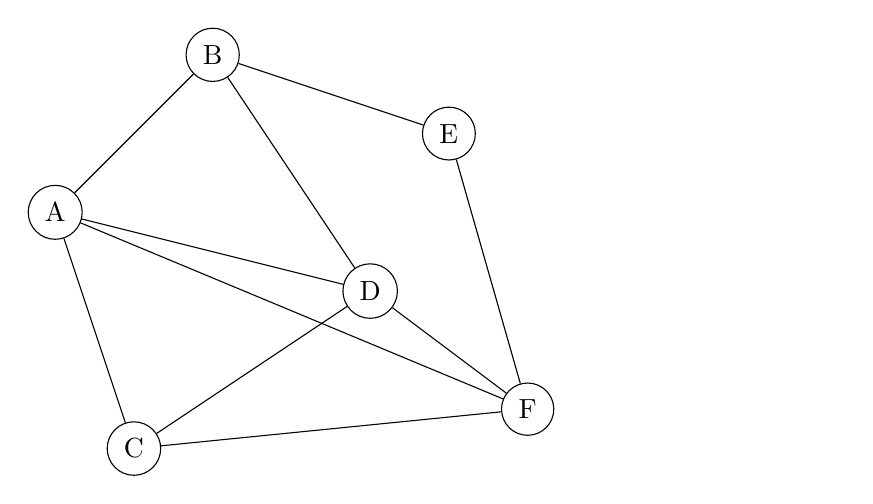
\begin{tikzpicture}
            \node[draw,circle] (A) at (0, 3) { A };
            \node[draw,circle] (B) at (2, 5) { B };
            \node[draw,circle] (C) at (1, 0) { C };
            \node[draw,circle] (D) at (4, 2) { D };
            \node[draw,circle] (E) at (5, 4) { E };
            \node[draw,circle] (F) at (6, 0.5) { F };

            \draw (A) to (B);
            \draw (A) to (C);
            \draw (D) to (C);
            \draw (E) to (B);
            \draw (A) -- (D);
            \draw (A) -- (F);
            \draw (B) -- (D);
            \draw (C) to (F);
            \draw (D) -- (F);
            \draw (E) -- (F);

            \draw[opacity=0,blue] (7, 5) -- (7.5, 5) node[anchor=west,black] { \scriptsize Caminho de A a F };

        \end{tikzpicture}

    \end{figure}

\end{frame}

\begin{frame}[fragile]{Visualização de um grafo conectado e caminhos}

    \begin{figure}
        \centering

        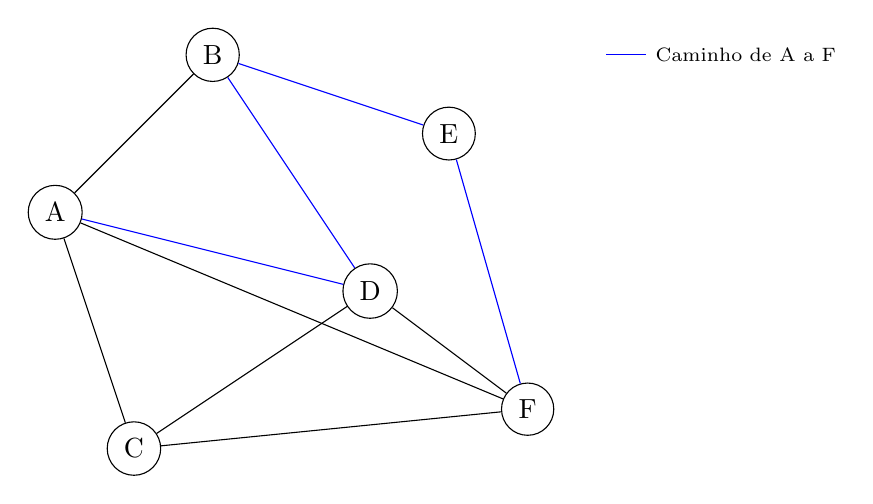
\begin{tikzpicture}
            \node[draw,circle] (A) at (0, 3) { A };
            \node[draw,circle] (B) at (2, 5) { B };
            \node[draw,circle] (C) at (1, 0) { C };
            \node[draw,circle] (D) at (4, 2) { D };
            \node[draw,circle] (E) at (5, 4) { E };
            \node[draw,circle] (F) at (6, 0.5) { F };

            \draw (A) to (B);
            \draw (A) to (C);
            \draw (D) to (C);
            \draw[blue] (E) to (B);
            \draw[blue] (A) -- (D);
            \draw (A) -- (F);
            \draw[blue] (B) -- (D);
            \draw (C) to (F);
            \draw (D) -- (F);
            \draw[blue] (E) -- (F);

            \draw[blue] (7, 5) -- (7.5, 5) node[anchor=west,black] { \scriptsize Caminho de A a F };

        \end{tikzpicture}

    \end{figure}

\end{frame}

\begin{frame}[fragile]{Visualização de um grafo conectado e caminhos}

    \begin{figure}
        \centering

        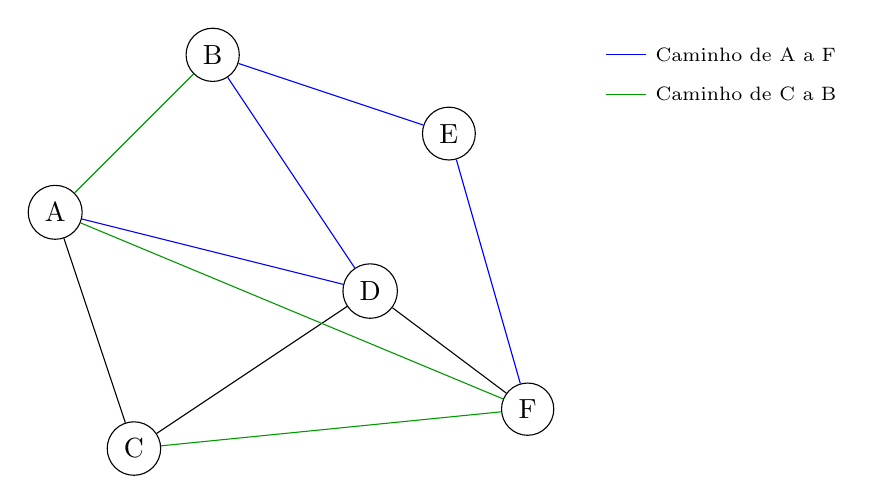
\begin{tikzpicture}
            \node[draw,circle] (A) at (0, 3) { A };
            \node[draw,circle] (B) at (2, 5) { B };
            \node[draw,circle] (C) at (1, 0) { C };
            \node[draw,circle] (D) at (4, 2) { D };
            \node[draw,circle] (E) at (5, 4) { E };
            \node[draw,circle] (F) at (6, 0.5) { F };

            \draw[green!60!black] (A) to (B);
            \draw (A) to (C);
            \draw (D) to (C);
            \draw[blue] (E) to (B);
            \draw[blue] (A) -- (D);
            \draw [green!60!black](A) -- (F);
            \draw[blue] (B) -- (D);
            \draw[green!60!black] (C) to (F);
            \draw (D) -- (F);
            \draw[blue] (E) -- (F);

            \draw[blue] (7, 5) -- (7.5, 5) node[anchor=west,black] { \scriptsize Caminho de A a F };
            \draw[green!60!black] (7, 4.5) -- (7.5, 4.5) node[anchor=west,black] { \scriptsize Caminho de C a B };

        \end{tikzpicture}

    \end{figure}

\end{frame}

\begin{frame}[fragile]{Visualização de um grafo conectado e caminhos}

    \begin{figure}
        \centering

        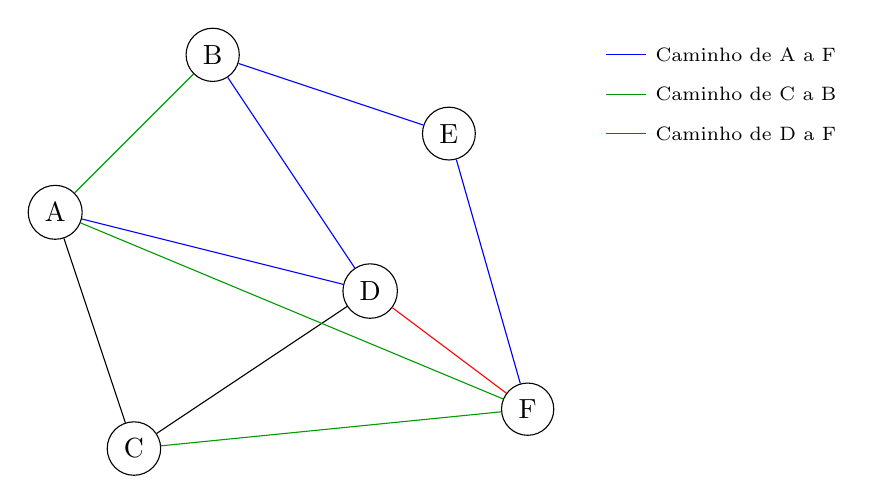
\begin{tikzpicture}
            \node[draw,circle] (A) at (0, 3) { A };
            \node[draw,circle] (B) at (2, 5) { B };
            \node[draw,circle] (C) at (1, 0) { C };
            \node[draw,circle] (D) at (4, 2) { D };
            \node[draw,circle] (E) at (5, 4) { E };
            \node[draw,circle] (F) at (6, 0.5) { F };

            \draw[green!60!black] (A) to (B);
            \draw (A) to (C);
            \draw (D) to (C);
            \draw[blue] (E) to (B);
            \draw[blue] (A) -- (D);
            \draw [green!60!black](A) -- (F);
            \draw[blue] (B) -- (D);
            \draw[green!60!black] (C) to (F);
            \draw[red] (D) -- (F);
            \draw[blue] (E) -- (F);

            \draw[blue] (7, 5) -- (7.5, 5) node[anchor=west,black] { \scriptsize Caminho de A a F };
            \draw[green!60!black] (7, 4.5) -- (7.5, 4.5) node[anchor=west,black] { \scriptsize Caminho de C a B };
            \draw[red] (7, 4) -- (7.5, 4) node[anchor=west,black] { \scriptsize Caminho de D a F };

        \end{tikzpicture}

    \end{figure}

\end{frame}



